\documentclass{report}[a4paper, 12pt]

\usepackage[left=0mm, top=0mm, bottom=0mm, right=0mm, margin=0mm]{geometry}
\usepackage{amsthm,tikz,subcaption}
\usetikzlibrary{arrows.meta}
\usetikzlibrary{arrows}
\usetikzlibrary{calc}
\usetikzlibrary{quotes,angles}

\usepackage{tkz-euclide}
\usetkzobj{all}

\begin{document}

    \begin{table}

        \begin{tabular}{ccc}

            % Step 1
            \begin{tikzpicture}
                \draw[-latex, dotted, draw=gray] (0,0)--(6,0) node [right] {$x$};
                \draw[-latex, dotted, draw=gray] (0,0)--(0,6) node [above] {$y$};
                \foreach \Point in {(3,4), (5,2), (4,4), (2,1), (5,5), (2,5)}{
                \node[circle,fill=black!60!green,inner sep=1.5pt,minimum size=3pt] at \Point {};
                }
                \draw [dotted, gray] (0,0) grid (6,6);
            \end{tikzpicture}

            &

            % Step 2
            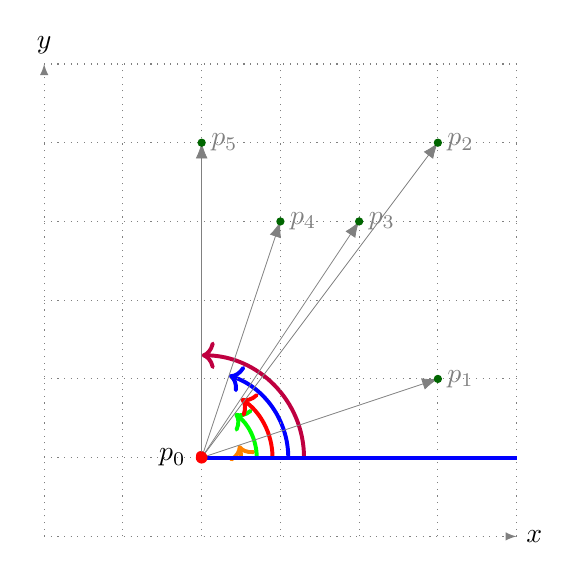
\begin{tikzpicture}
                \draw[-latex, dotted, draw=gray] (0,0)--(6,0) node [right] {$x$};
                \draw[-latex, dotted, draw=gray] (0,0)--(0,6) node [above] {$y$};

                \coordinate (a) at (5,1);
                \coordinate (b) at (2,1);
                \coordinate (c) at (5,2);
                \pic [draw, ->, "",draw=orange, angle eccentricity=1.5,angle radius=0.5cm,line width=0.5mm] {angle=a--b--c};

                \coordinate (a) at (5,1);
                \coordinate (b) at (2,1);
                \coordinate (c) at (5,5);
                \pic [draw, ->, "",draw=green, angle eccentricity=1.5,angle radius=0.7cm,line width=0.5mm] {angle=a--b--c};

                \coordinate (a) at (4,1);
                \coordinate (b) at (2,1);
                \coordinate (c) at (4,4);
                \pic [draw, ->, "",draw=red, angle eccentricity=1.5,angle radius=0.9cm,line width=0.5mm] {angle=a--b--c};

                \coordinate (a) at (3,1);
                \coordinate (b) at (2,1);
                \coordinate (c) at (3,4);
                \pic [draw, ->, "",draw=blue, angle eccentricity=1.5,angle radius=1.1cm,line width=0.5mm] {angle=a--b--c};

                \coordinate (a) at (3,1);
                \coordinate (b) at (2,1);
                \coordinate (c) at (2,5);
                \pic [draw, ->, "",draw=purple, angle eccentricity=1.5,angle radius=1.3cm,line width=0.5mm] {angle=a--b--c};

                \draw [dotted, gray] (0,0) grid (6,6);
                \node [red] at (2,1) {\textbullet};
                \draw [line width=0.5mm, blue, domain=2:6, samples=100] plot(\x, {((1)});

                \foreach \Point [count=\i] in {(5,2), (5,5), (4,4), (3,4), (2,5)}{

                \draw[-{Latex[length=2mm]},line width=0.1mm,gray] (2, 1) -- \Point node[right]{$p_\i$};
                }

                \foreach \Point in {(5,2), (5,5), (4,4), (3,4), (2,5), (2,1)}{
                \node[circle,fill=black!60!green,inner sep=1pt,minimum size=3pt] at \Point {};
                }

                \node[circle,inner sep=1.5pt,fill=red,label=left:{$p_0$}] at (2,1) {};
                %\node[circle,inner sep=1.5pt,fill=red,label=left:{$q$}] at (5,2) {};

            \end{tikzpicture}

            &

            % Step 3
            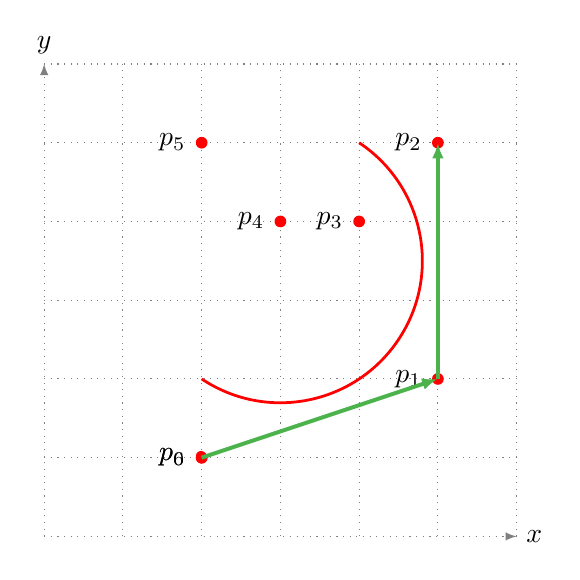
\begin{tikzpicture}[my_arrow/.style={decorate,decoration={markings,mark=at position 1 with {\arrow[scale=1]{>}};}}]
                \draw[-latex, dotted, draw=gray] (0,0)--(6,0) node [right] {$x$};
                \draw[-latex, dotted, draw=gray] (0,0)--(0,6) node [above] {$y$};

                \draw [dotted, gray] (0,0) grid (6,6);
                \node [red] at (2,1) {\textbullet};

                \foreach \Point [count=\i] in {(5,2), (5,5), (4,4), (3,4), (2,5), (2,1)}{
                \node[circle,fill=black!60!green,inner sep=1pt,minimum size=3pt] at \Point {};
                \node[circle,inner sep=1.5pt,fill=red,label=left:{$p_\i$}] at \Point {};
                }

                \node[circle,inner sep=1.5pt,fill=red,label=left:{$p_0$}] at (2,1) {};

                \draw[-{Latex[length=2mm]},line width=0.5mm,green!40!gray] (2, 1) -- (5, 2);
                \draw[-{Latex[length=2mm]},line width=0.5mm,green!40!gray] (5, 2) -- (5, 5);

                \tkzDefPoint(2,2){A}
                \tkzDefPoint(4,2){B}
                \tkzDefPoint(4,5){C}
                \tkzCircumCenter(A,B,C)
                \tkzGetPoint{O}
                \tkzDrawArc[draw=red,postaction={my_arrow},line width=1pt](O,A)(C)

            \end{tikzpicture}

            \\

            % Step 4
            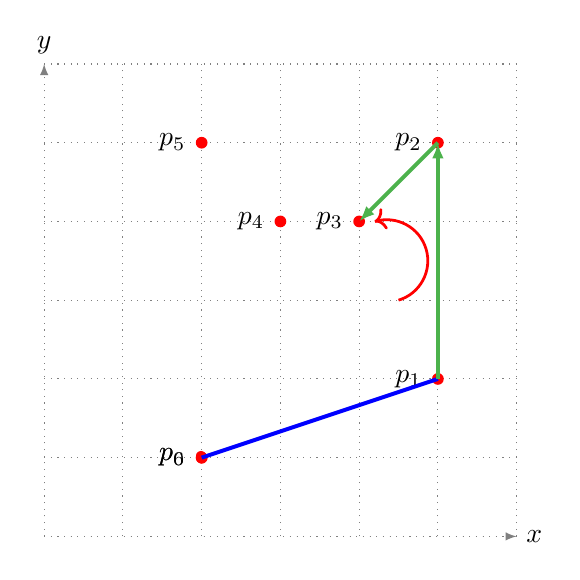
\begin{tikzpicture}[my_arrow/.style={decorate,decoration={markings,mark=at position 1 with {\arrow[scale=1]{>}};}}]
                \draw[-latex, dotted, draw=gray] (0,0)--(6,0) node [right] {$x$};
                \draw[-latex, dotted, draw=gray] (0,0)--(0,6) node [above] {$y$};

                \draw [dotted, gray] (0,0) grid (6,6);
                \node [red] at (2,1) {\textbullet};

                \foreach \Point [count=\i] in {(5,2), (5,5), (4,4), (3,4), (2,5), (2,1)}{
                \node[circle,fill=black!60!green,inner sep=1pt,minimum size=3pt] at \Point {};
                \node[circle,inner sep=1.5pt,fill=red,label=left:{$p_\i$}] at \Point {};
                }

                \node[circle,inner sep=1.5pt,fill=red,label=left:{$p_0$}] at (2,1) {};

                \draw [line width=0.5mm, draw=blue] (2,1) -- (5,2);

                \draw[-{Latex[length=2mm]},line width=0.5mm,green!40!gray] (5, 2) -- (5, 5);
                \draw[-{Latex[length=2mm]},line width=0.5mm,green!40!gray] (5, 5) -- (4, 4);

                \tkzDefPoint(4.5,3){A}
                \tkzDefPoint(4.5,4){B}
                \tkzDefPoint(4.2,4){C}
                \tkzCircumCenter(A,B,C)
                \tkzGetPoint{O}
                \tkzDrawArc[draw=red,postaction={my_arrow},line width=1pt](O,A)(C)

            \end{tikzpicture}

            &

            % Step 5
            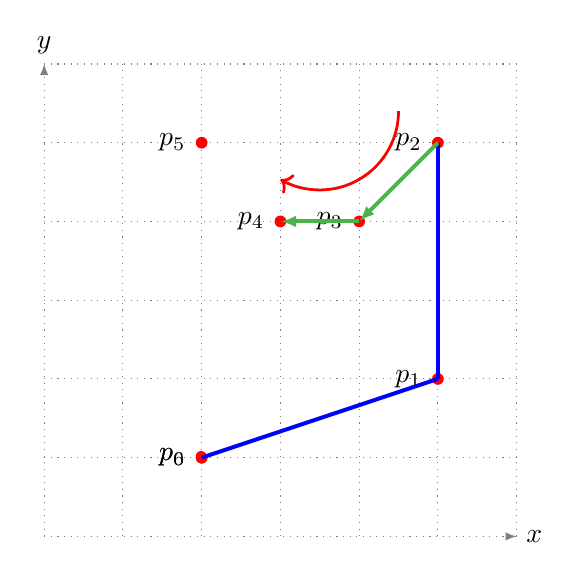
\begin{tikzpicture}
                \draw[-latex, dotted, draw=gray] (0,0)--(6,0) node [right] {$x$};
                \draw[-latex, dotted, draw=gray] (0,0)--(0,6) node [above] {$y$};

                \draw [dotted, gray] (0,0) grid (6,6);
                \node [red] at (2,1) {\textbullet};

                \foreach \Point [count=\i] in {(5,2), (5,5), (4,4), (3,4), (2,5), (2,1)}{
                \node[circle,fill=black!60!green,inner sep=1pt,minimum size=3pt] at \Point {};
                \node[circle,inner sep=1.5pt,fill=red,label=left:{$p_\i$}] at \Point {};
                }

                \node[circle,inner sep=1.5pt,fill=red,label=left:{$p_0$}] at (2,1) {};

                \draw [line width=0.5mm, draw=blue] (2,1) -- (5,2);
                \draw [line width=0.5mm, draw=blue] (5,2) -- (5,5);

                \draw[-{Latex[length=2mm]},line width=0.5mm,green!40!gray] (5, 5) -- (4, 4);
                \draw[-{Latex[length=2mm]},line width=0.5mm,green!40!gray] (4, 4) -- (3, 4);

                \draw[draw=red,ultra thick,line width=1pt, ->] (4.5,5.4) arc (0:-120:1);

            \end{tikzpicture}

            &
            % Step 6
            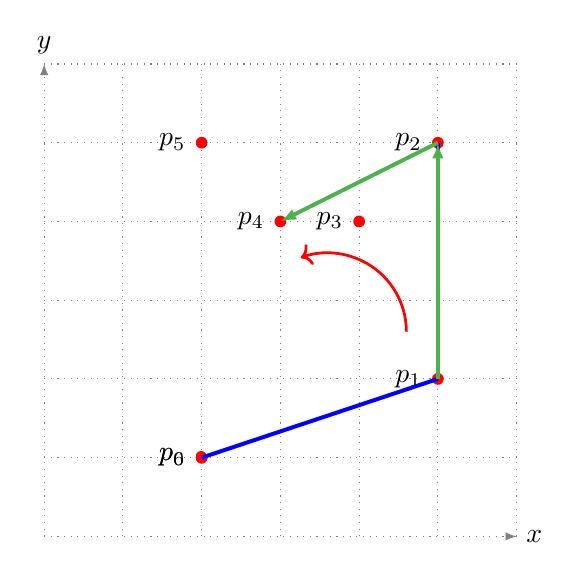
\begin{tikzpicture}
                \draw[-latex, dotted, draw=gray] (0,0)--(6,0) node [right] {$x$};
                \draw[-latex, dotted, draw=gray] (0,0)--(0,6) node [above] {$y$};

                \draw [dotted, gray] (0,0) grid (6,6);
                \node [red] at (2,1) {\textbullet};

                \foreach \Point [count=\i] in {(5,2), (5,5), (4,4), (3,4), (2,5), (2,1)}{
                \node[circle,fill=black!60!green,inner sep=1pt,minimum size=3pt] at \Point {};
                \node[circle,inner sep=1.5pt,fill=red,label=left:{$p_\i$}] at \Point {};
                }

                \node[circle,inner sep=1.5pt,fill=red,label=left:{$p_0$}] at (2,1) {};

                \draw [line width=0.5mm, draw=blue] (2,1) -- (5,2);
                \draw [line width=0.5mm, draw=blue] (5,2) -- (5,5);

                \draw[-{Latex[length=2mm]},line width=0.5mm,green!40!gray] (5, 2) -- (5, 5);
                \draw[-{Latex[length=2mm]},line width=0.5mm,green!40!gray] (5, 5) -- (3, 4);

                \draw[draw=red,ultra thick,line width=1pt, ->] (4.6,2.6) arc (0:110:1);

            \end{tikzpicture}

            \\

            % Step 7
            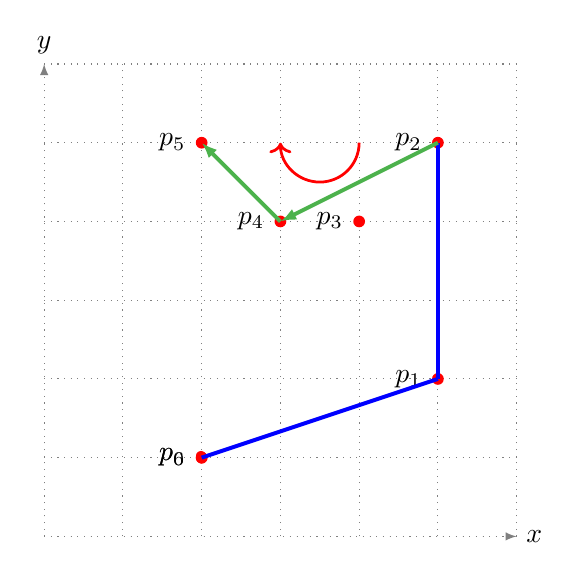
\begin{tikzpicture}
                \draw[-latex, dotted, draw=gray] (0,0)--(6,0) node [right] {$x$};
                \draw[-latex, dotted, draw=gray] (0,0)--(0,6) node [above] {$y$};

                \draw [dotted, gray] (0,0) grid (6,6);
                \node [red] at (2,1) {\textbullet};

                \foreach \Point [count=\i] in {(5,2), (5,5), (4,4), (3,4), (2,5), (2,1)}{
                \node[circle,fill=black!60!green,inner sep=1pt,minimum size=3pt] at \Point {};
                \node[circle,inner sep=1.5pt,fill=red,label=left:{$p_\i$}] at \Point {};
                }

                \node[circle,inner sep=1.5pt,fill=red,label=left:{$p_0$}] at (2,1) {};

                \draw [line width=0.5mm, draw=blue] (2,1) -- (5,2);
                \draw [line width=0.5mm, draw=blue] (5,2) -- (5,5);

                \draw[-{Latex[length=2mm]},line width=0.5mm,green!40!gray] (5, 5) -- (3, 4);
                \draw[-{Latex[length=2mm]},line width=0.5mm,green!40!gray] (3, 4) -- (2, 5);

                \draw[draw=red,ultra thick,line width=1pt, ->] (4,5) arc (0:-180:0.5);

            \end{tikzpicture}

            &

            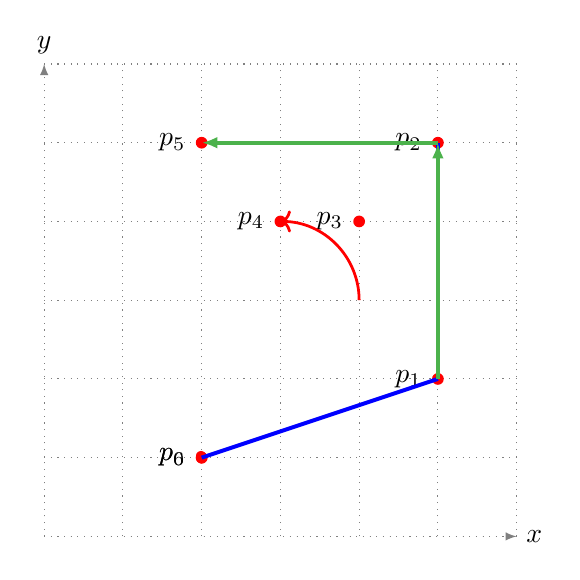
\begin{tikzpicture}
                \draw[-latex, dotted, draw=gray] (0,0)--(6,0) node [right] {$x$};
                \draw[-latex, dotted, draw=gray] (0,0)--(0,6) node [above] {$y$};

                \draw [dotted, gray] (0,0) grid (6,6);
                \node [red] at (2,1) {\textbullet};

                \foreach \Point [count=\i] in {(5,2), (5,5), (4,4), (3,4), (2,5), (2,1)}{
                \node[circle,fill=black!60!green,inner sep=1pt,minimum size=3pt] at \Point {};
                \node[circle,inner sep=1.5pt,fill=red,label=left:{$p_\i$}] at \Point {};
                }

                \node[circle,inner sep=1.5pt,fill=red,label=left:{$p_0$}] at (2,1) {};

                \draw [line width=0.5mm, draw=blue] (2,1) -- (5,2);
                \draw [line width=0.5mm, draw=blue] (5,2) -- (5,5);

                \draw[-{Latex[length=2mm]},line width=0.5mm,green!40!gray] (5, 2) -- (5, 5);
                \draw[-{Latex[length=2mm]},line width=0.5mm,green!40!gray] (5, 5) -- (2, 5);

                \draw[draw=red,ultra thick,line width=1pt, ->] (4,3) arc (0:90:1);

            \end{tikzpicture}

            &

            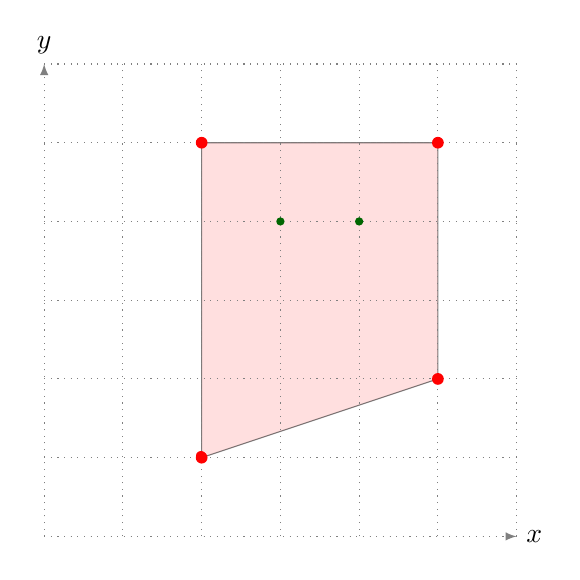
\begin{tikzpicture}
                \draw[-latex, dotted, draw=gray] (0,0)--(6,0) node [right] {$x$};
                \draw[-latex, dotted, draw=gray] (0,0)--(0,6) node [above] {$y$};

                \node (v1) at (2,1) {};
                \node (v2) at (5,2) {};
                \node (v3) at (5,5) {};
                \node (v4) at (2,5) {};
                \draw[opacity=0.5,fill=pink] (v1.center)--(v2.center)--(v3.center)--(v4.center)--(v1.center);

                \draw [dotted, gray] (0,0) grid (6,6);
                \node [red] at (2,1) {\textbullet};

                \foreach \Point in {(3,4), (5,2), (4,4), (2,1), (5,5), (2,5)}{
                \node[circle,fill=black!60!green,inner sep=1pt,minimum size=3pt] at \Point {};
                }

                \node[circle,inner sep=1.5pt,fill=red,label=left:{}] at (2,1) {};
                \node[circle,inner sep=1.5pt,fill=red,label=left:{}] at (5,2) {};
                \node[circle,inner sep=1.5pt,fill=red,label=left:{}] at (5,5) {};
                \node[circle,inner sep=1.5pt,fill=red,label=left:{}] at (2,5) {};

            \end{tikzpicture}

        \end{tabular}

    \end{table}

\end{document}